%=====================================================================
%  final_diagram_gallery.tex
%  Five candidate designs for the Final Conceptual Diagram of
%  homological_understanding.tex  (X = P^1_C = S^2).
%  Compile:  latexmk -pdf final_diagram_gallery.tex
%  No shell-escape, no external images, no nonstandard fonts.
%=====================================================================
\documentclass[11pt]{article}

\usepackage[T1]{fontenc}
\usepackage{lmodern}
\usepackage[a4paper,margin=2.0cm]{geometry}
\usepackage{amsmath,amssymb,amsthm,mathtools}
\usepackage{tikz}
\usepackage{tikz-cd}
\usepackage{xcolor}
\usepackage{enumitem}
\usepackage{array}
\usepackage{booktabs}

\usetikzlibrary{arrows.meta,positioning,calc,fit,backgrounds,
  decorations.markings,decorations.pathmorphing,decorations.pathreplacing}

%---------------------------------------------------------------------
\definecolor{inkblue}{RGB}{22,32,72}
\definecolor{polered}{RGB}{172,28,40}
\definecolor{zerogreen}{RGB}{18,108,72}
\definecolor{accent}{RGB}{176,104,12}
\definecolor{paper}{RGB}{250,248,240}
\definecolor{faint}{RGB}{120,120,132}

%---------------------------------------------------------------------
\newcommand{\CC}{\mathbb C}
\newcommand{\RR}{\mathbb R}
\newcommand{\ZZ}{\mathbb Z}
\newcommand{\PP}{\mathbb P}
\newcommand{\OO}{\mathcal O}
\newcommand{\dR}{\mathrm{dR}}
\newcommand{\im}{\operatorname{im}}
\newcommand{\kerop}{\operatorname{ker}}
\newcommand{\Pic}{\operatorname{Pic}}

%---------------------------------------------------------------------
%  Shared gallery styles
%---------------------------------------------------------------------
\tikzset{
  >=Stealth,
  absb/.style={draw=inkblue, rounded corners=2pt, fill=paper, align=center,
               inner sep=4pt, font=\footnotesize, text=inkblue},
  geob/.style={draw=zerogreen, rounded corners=2pt, fill=paper, align=center,
               inner sep=4pt, font=\footnotesize, text=inkblue},
  delb/.style={draw=polered, line width=1.1pt, rounded corners=2pt, fill=paper,
               align=center, inner sep=5pt, font=\footnotesize\bfseries, text=polered},
  aar/.style={->, inkblue, line width=0.7pt},
  gar/.style={->, zerogreen, line width=0.7pt},
  dar/.style={->, polered, line width=0.9pt},
  rung/.style={densely dotted, faint, line width=0.6pt},
  glab/.style={font=\scriptsize\itshape, text=faint, fill=paper, inner sep=1pt},
}
% small schematic sphere (radius 1; scale the enclosing scope to resize)
\newcommand{\spherepic}{%
  \begin{scope}\clip (0,0) circle (1);
    \fill[zerogreen, fill opacity=0.13] (-1,-1) rectangle (1,0.28);
    \fill[polered,  fill opacity=0.11] (-1,-0.28) rectangle (1,1);
    \fill[accent,   fill opacity=0.42] (-1,-0.28) rectangle (1,0.28);
  \end{scope}
  \draw[inkblue, line width=0.6pt] (0,0) circle (1);
  \draw[inkblue, dashed, line width=0.35pt] (1,0) arc[start angle=0,end angle=180,x radius=1,y radius=0.24];
  \draw[inkblue, line width=0.5pt] (1,0) arc[start angle=0,end angle=-180,x radius=1,y radius=0.24];
}
\newcommand{\optcap}[1]{\par\smallskip{\centering\footnotesize\textit{#1}\par}\medskip}

%---------------------------------------------------------------------
\title{\bfseries Final Conceptual Diagram --- Five Candidate Designs}
\author{\textsc{A Comparison Gallery}}
\date{\today}
%---------------------------------------------------------------------

\begin{document}
\maketitle

\noindent This gallery draws five candidate designs for the closing
\emph{Final Conceptual Diagram} of \texttt{homological\_\allowbreak understanding.tex}, whose
subject is $X=\PP^1_\CC$, read at once as the $2$-sphere $S^2$ and as a complex
curve. The pipeline to synthesize is
\begin{center}
\resizebox{\textwidth}{!}{$\displaystyle
  \text{local data}\to\text{chain complex }(C^\bullet,d^2{=}0)\to
  \text{cohomology }H^n\to 0{\to}A{\to}B{\to}C{\to}0\to
  \text{LES}\xrightarrow{\ \delta\ }\text{global class}$}
\end{center}
with the Mayer--Vietoris realization
\[
  0\to\Omega^\bullet(\PP^1)\to\Omega^\bullet(U_0)\oplus\Omega^\bullet(U_\infty)
   \to\Omega^\bullet(\CC^\times)\to0
\]
($U_0\cap U_\infty=\CC^\times\simeq S^1$,\ $\delta^1\colon H^1(\CC^\times)
\xrightarrow{\cong}H^2(\PP^1)$,\ $\Pic(\PP^1)=\ZZ$).

\begin{center}\footnotesize
\textcolor{inkblue}{\rule{9pt}{7pt}}\ abstract construction\qquad
\textcolor{zerogreen}{\rule{9pt}{7pt}}\ geometry / Mayer--Vietoris\qquad
\textcolor{polered}{\rule{9pt}{7pt}}\ $\delta$ / obstruction
\end{center}

%=====================================================================
\section*{Option 1: Two-track ``abstraction $\leftrightarrow$ instance'' ladder}
%=====================================================================
\begin{center}
\resizebox{\textwidth}{!}{%
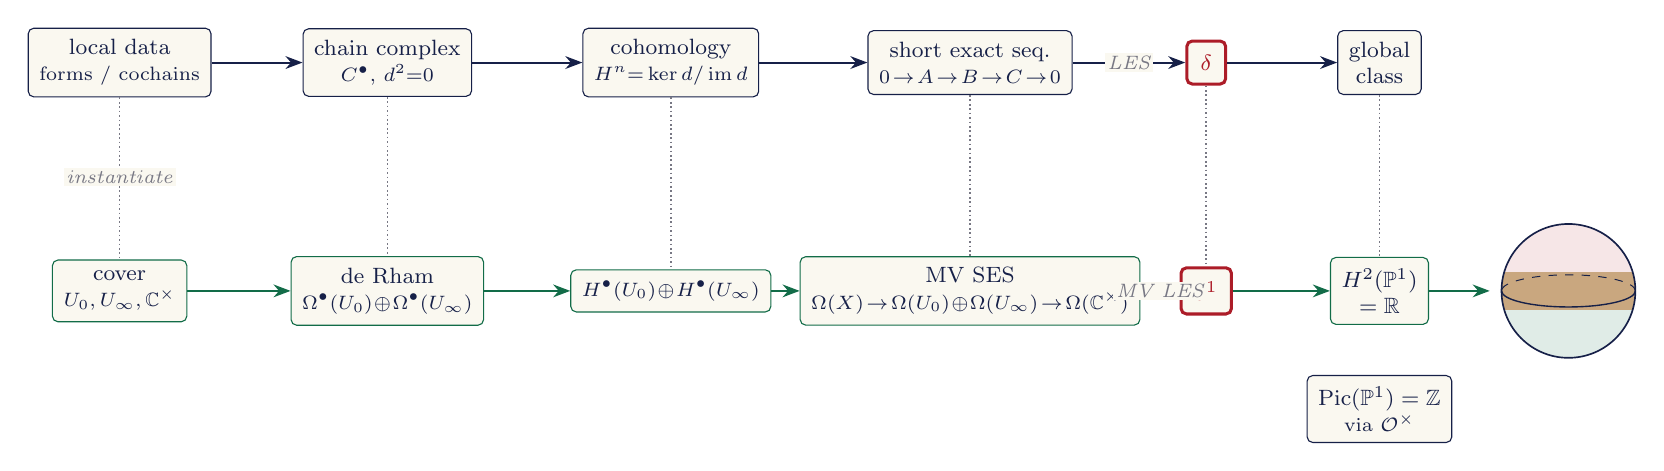
\begin{tikzpicture}
  % ---- abstract rail (top) ----
  \node[absb] (a1) at (0,0)    {local data\\ \scriptsize forms / cochains};
  \node[absb] (a2) at (3.4,0)  {chain complex\\ \scriptsize $C^\bullet,\,d^2{=}0$};
  \node[absb] (a3) at (7.0,0)  {cohomology\\ \scriptsize $H^n{=}\kerop d/\im d$};
  \node[absb] (a4) at (10.8,0) {short exact seq.\\ \scriptsize $0\!\to\!A\!\to\!B\!\to\!C\!\to\!0$};
  \node[delb] (a5) at (13.8,0) {$\delta$};
  \node[absb] (a6) at (16.0,0) {global\\ class};
  \draw[aar] (a1)--(a2); \draw[aar] (a2)--(a3); \draw[aar] (a3)--(a4);
  \draw[aar] (a4)--(a5) node[glab,midway]{LES}; \draw[aar] (a5)--(a6);
  % ---- concrete rail (bottom) ----
  \node[geob] (c1) at (0,-2.9)    {cover\\ \scriptsize $U_0,U_\infty,\CC^\times$};
  \node[geob] (c2) at (3.4,-2.9)  {de Rham\\ \scriptsize $\Omega^\bullet(U_0)\!\oplus\!\Omega^\bullet(U_\infty)$};
  \node[geob] (c3) at (7.0,-2.9)  {\scriptsize $H^\bullet(U_0)\!\oplus\!H^\bullet(U_\infty)$};
  \node[geob] (c4) at (10.8,-2.9) {MV SES\\ \scriptsize $\Omega(X)\!\to\!\Omega(U_0)\!\oplus\!\Omega(U_\infty)\!\to\!\Omega(\CC^\times)$};
  \node[delb] (c5) at (13.8,-2.9) {$\delta^1$};
  \node[geob] (c6) at (16.0,-2.9) {$H^2(\PP^1)$\\ $=\RR$};
  \draw[gar] (c1)--(c2); \draw[gar] (c2)--(c3); \draw[gar] (c3)--(c4);
  \draw[gar] (c4)--(c5) node[glab,midway]{MV LES}; \draw[gar] (c5)--(c6);
  % ---- instantiation rungs ----
  \foreach \t/\b in {a1/c1,a2/c2,a3/c3,a4/c4,a5/c5,a6/c6}{ \draw[rung] (\t)--(\b); }
  \node[glab] at (-0.0,-1.45) {instantiate};
  % ---- payoff terminus ----
  \node[absb] at (16.0,-4.4) {$\Pic(\PP^1)=\ZZ$\\ \scriptsize via $\OO^\times$};
  \begin{scope}[shift={(18.4,-2.9)}, scale=0.85]\spherepic\end{scope}
  \draw[gar] (c6) -- (17.4,-2.9);
\end{tikzpicture}}
\end{center}
\optcap{\textbf{Best for}: showing the document's thesis --- one abstract machine,
instantiated on $\PP^1$ --- as the literal structure; single left-to-right reading,
$\delta$ as the shared climax, geometric payoff at the end. \textbf{Trade-off}:
the widest design (needs full-width scaling).}

%=====================================================================
\section*{Option 2: The ``$\delta$-funnel'' (the connecting map as the lens)}
%=====================================================================
\begin{center}
\resizebox{0.92\textwidth}{!}{%
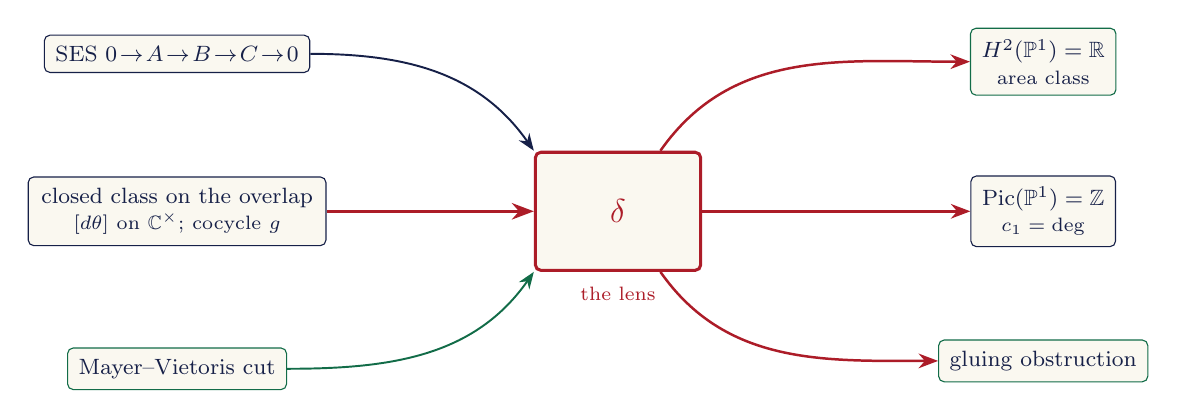
\begin{tikzpicture}
  \node[delb, font=\large\bfseries, minimum width=2.1cm, minimum height=1.5cm] (d) at (0,0) {$\delta$};
  \node[font=\scriptsize, text=polered] at (0,-1.05) {the lens};
  % left inputs
  \node[absb, text width=3.5cm] (in) at (-5.6,0) {closed class on the overlap\\ \scriptsize $[d\theta]$ on $\CC^\times$;\ cocycle $g$};
  \node[absb] (ses) at (-5.6,2.0) {SES $0\!\to\!A\!\to\!B\!\to\!C\!\to\!0$};
  \node[geob] (mv)  at (-5.6,-2.0) {Mayer--Vietoris cut};
  \draw[dar, line width=1.1pt] (in)--(d);
  \draw[aar] (ses) to[out=0,in=125] (d.north west);
  \draw[gar] (mv)  to[out=0,in=-125] (d.south west);
  % right fan-out
  \node[geob] (h2)   at (5.4,1.9)  {$H^2(\PP^1)=\RR$\\ \scriptsize area class};
  \node[absb] (pic)  at (5.4,0)    {$\Pic(\PP^1)=\ZZ$\\ \scriptsize $c_1=\deg$};
  \node[geob] (glue) at (5.4,-1.9) {gluing obstruction};
  \draw[dar] (d) to[out=55,in=180]  (h2);
  \draw[dar] (d) -- (pic);
  \draw[dar] (d) to[out=-55,in=180] (glue);
\end{tikzpicture}}
\end{center}
\optcap{\textbf{Best for}: dramatizing the title \emph{Exactness as a Lens} --- one
construction ($\delta$) drives every result in the document. \textbf{Trade-off}:
de-emphasizes the upstream pipeline (chain complex $\to$ cohomology).}

%=====================================================================
\section*{Option 3: Geometry-anchored hub}
%=====================================================================
\begin{center}
\resizebox{0.95\textwidth}{!}{%
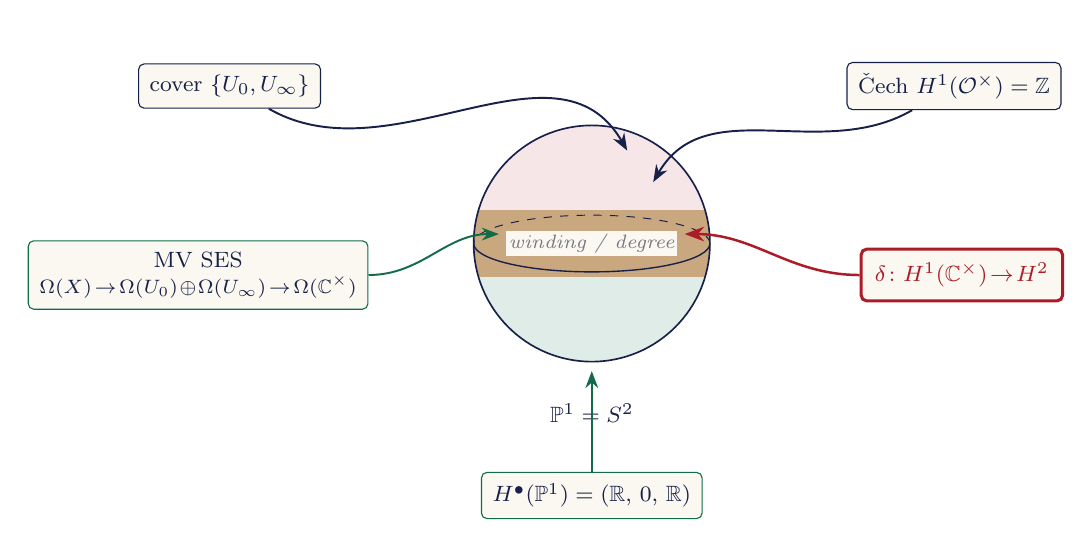
\begin{tikzpicture}
  \begin{scope}[scale=1.5]\spherepic\end{scope}
  \node[inkblue, font=\footnotesize] at (0,-2.15) {$\PP^1=S^2$};
  % satellites
  \node[absb] (cov) at (-4.6,2.0)  {cover $\{U_0,U_\infty\}$};
  \node[geob] (mv)  at (-5.0,-0.4) {MV SES\\ \scriptsize $\Omega(X)\!\to\!\Omega(U_0)\!\oplus\!\Omega(U_\infty)\!\to\!\Omega(\CC^\times)$};
  \node[delb] (del) at (4.7,-0.4)  {$\delta\colon H^1(\CC^\times)\!\to\!H^2$};
  \node[absb] (pic) at (4.6,2.0)   {\v Cech $H^1(\OO^\times)=\ZZ$};
  \node[geob] (coh) at (0,-3.2)    {$H^\bullet(\PP^1)=(\RR,\,0,\,\RR)$};
  % arrows pointing AT features (with reads-off semantics)
  \draw[aar] (cov) to[out=-30,in=120] (0.45,1.18) node[glab,pos=0.62]{the two caps};
  \draw[gar] (mv)  to[out=0,in=180]   (-1.18,0.12) node[glab,pos=0.7]{the overlap band};
  \draw[dar] (del) to[out=180,in=0]   (1.18,0.12) node[glab,pos=0.62,text=polered]{the area class};
  \draw[aar] (pic) to[out=-150,in=60] (0.78,0.78) node[glab,pos=0.6]{winding / degree};
  \draw[gar] (coh) -- (0,-1.62);
\end{tikzpicture}}
\end{center}
\optcap{\textbf{Best for}: maximal fusion of algebra and the document's geometry ---
each tool visibly \emph{reads off} a feature of the sphere. \textbf{Trade-off}: a
hub layout (rather than a pipeline); only justified because the hub is a concrete
object and every arrow carries a stated ``reads-off'' meaning.}

%=====================================================================
\section*{Option 4: Vertical ``abstraction tower''}
%=====================================================================
\begin{center}
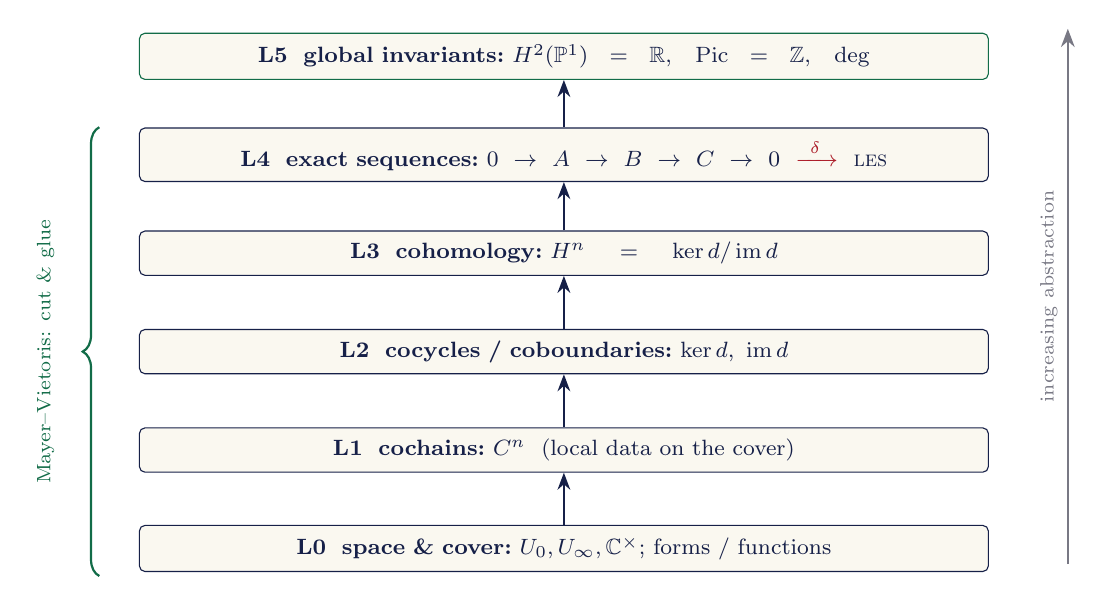
\begin{tikzpicture}[x=1cm,y=1cm]
  \def\W{10.5}
  \node[absb, text width=\W cm] (l0) at (0,0)   {\textbf{L0 \ space \& cover:}\ $U_0,U_\infty,\CC^\times$;\ forms / functions};
  \node[absb, text width=\W cm] (l1) at (0,1.25){\textbf{L1 \ cochains:}\ $C^n$ \ (local data on the cover)};
  \node[absb, text width=\W cm] (l2) at (0,2.5) {\textbf{L2 \ cocycles / coboundaries:}\ $\kerop d,\ \im d$};
  \node[absb, text width=\W cm] (l3) at (0,3.75){\textbf{L3 \ cohomology:}\ $H^n=\kerop d/\im d$};
  \node[absb, text width=\W cm] (l4) at (0,5.0) {\textbf{L4 \ exact sequences:}\ $0\!\to\!A\!\to\!B\!\to\!C\!\to\!0$\ \ {\color{polered}$\xrightarrow{\ \delta\ }$}\ \ \textsc{les}};
  \node[geob, text width=\W cm] (l5) at (0,6.25){\textbf{L5 \ global invariants:}\ $H^2(\PP^1)=\RR$,\quad $\Pic=\ZZ$,\quad $\deg$};
  \foreach \a/\b in {l0/l1,l1/l2,l2/l3,l3/l4,l4/l5}{ \draw[aar] (\a)--(\b); }
  % abstraction axis
  \draw[->, faint, line width=0.8pt] (6.4,-0.2)--(6.4,6.6) node[midway, right, rotate=90, anchor=south, font=\scriptsize]{increasing abstraction};
  % Mayer-Vietoris side bracket spanning L0..L4
  \draw[decorate, decoration={brace, amplitude=6pt}, zerogreen, line width=0.8pt]
        (-5.9,-0.35) -- (-5.9,5.35);
  \node[zerogreen, font=\scriptsize, rotate=90, anchor=south] at (-6.35,2.5)
        {Mayer--Vietoris: cut \& glue};
\end{tikzpicture}
\end{center}
\optcap{\textbf{Best for}: a clean, page-friendly ladder of abstraction read
bottom-to-top, ending in the concrete invariants. \textbf{Trade-off}: the
``cut and glue'' Mayer--Vietoris story survives only as a side annotation.}

%=====================================================================
\section*{Option 5: The zigzag as the literal spine}
%=====================================================================
\begin{center}
\resizebox{0.86\textwidth}{!}{%
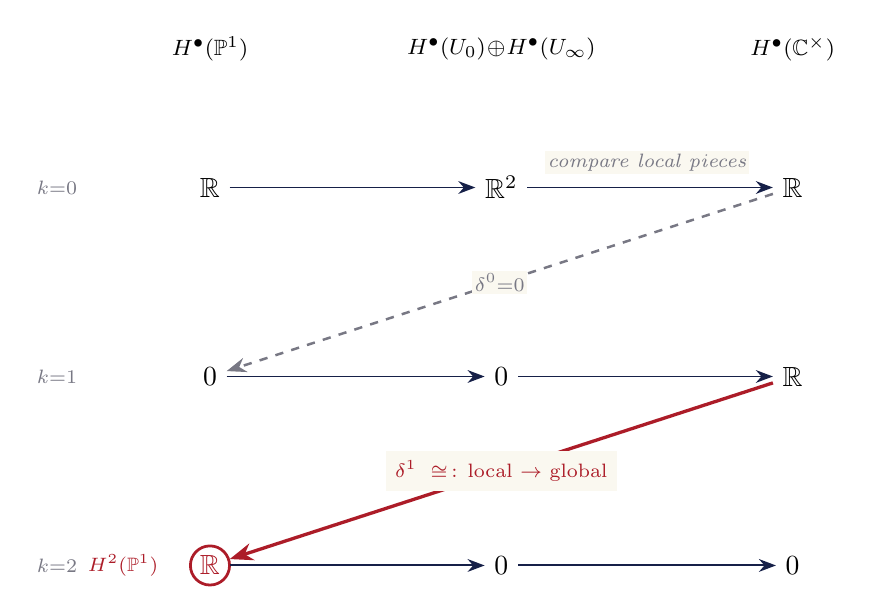
\begin{tikzpicture}[x=1.85cm,y=1.6cm]
  \node[font=\footnotesize] at (0,1.1) {$H^\bullet(\PP^1)$};
  \node[font=\footnotesize] at (2,1.1) {$H^\bullet(U_0)\!\oplus\!H^\bullet(U_\infty)$};
  \node[font=\footnotesize] at (4,1.1) {$H^\bullet(\CC^\times)$};
  \node[faint, font=\scriptsize] at (-1.05,0)    {$k{=}0$};
  \node[faint, font=\scriptsize] at (-1.05,-1.5) {$k{=}1$};
  \node[faint, font=\scriptsize] at (-1.05,-3.0) {$k{=}2$};
  \node (X0) at (0,0) {$\RR$};  \node (M0) at (2,0) {$\RR^2$}; \node (V0) at (4,0) {$\RR$};
  \node (X1) at (0,-1.5) {$0$}; \node (M1) at (2,-1.5) {$0$};  \node (V1) at (4,-1.5) {$\RR$};
  \node[text=polered] (X2) at (0,-3.0) {$\RR$}; \node (M2) at (2,-3.0) {$0$}; \node (V2) at (4,-3.0) {$0$};
  \node[circle, draw=polered, line width=1pt, inner sep=5pt] at (X2) {};
  \node[font=\scriptsize, text=polered, left=8pt] at (X2.west) {$H^2(\PP^1)$};
  \foreach \a/\b/\c in {X0/M0/V0, X1/M1/V1, X2/M2/V2}{
    \draw[aar] (\a)--(\b); \draw[aar] (\b)--(\c); }
  \node[glab] at (3,0.2) {compare local pieces};
  \draw[dar, faint, dashed] (V0)--(X1) node[glab, pos=0.5]{$\delta^0{=}0$};
  \draw[dar, line width=1.2pt] (V1)--(X2)
        node[pos=0.5, fill=paper, font=\scriptsize, text=polered]{$\delta^1\ \cong$\,: local $\to$ global};
\end{tikzpicture}}
\end{center}
\optcap{\textbf{Best for}: making the connecting map's zigzag the visible backbone,
rhyming with the document's staircase figure. \textbf{Trade-off}: overlaps heavily
with an existing figure, so it adds the least \emph{new} information.}

%=====================================================================
\section*{Comparison}
%=====================================================================
\begin{center}\footnotesize
\renewcommand{\arraystretch}{1.3}
\begin{tabular}{@{}p{1.5cm} p{3.0cm} p{2.3cm} p{3.0cm} p{3.0cm}@{}}
\toprule
\textbf{Option} & \textbf{Idea} & \textbf{Reading} & \textbf{Best for} & \textbf{Trade-off}\\
\midrule
1. Ladder & abstract rail $\parallel$ $\PP^1$ rail, joined by rungs & left $\to$ right, two rows &
  the thesis ``machine, then instance''; ends in geometry & widest design\\
2. Funnel & $\delta$ as a central lens; inputs in, results out & converge $\to$ fan out &
  the title \emph{Exactness as a Lens} & hides the upstream pipeline\\
3. Hub & sphere at center; tools read off its features & radial, inward arrows &
  fusing algebra with the geometry & not a pipeline (hub layout)\\
4. Tower & strata from concrete to abstract & bottom $\to$ top &
  the ladder of abstraction; compact & MV only a side note\\
5. Spine & the LES staircase as backbone & zigzag &
  the snake as the visible spine & duplicates an existing figure\\
\bottomrule
\end{tabular}
\end{center}

\medskip
\noindent\textbf{Recommendation.}\ \emph{Option~1 (the two-track ladder)} is the
strongest \emph{final synthesis}: it makes the document's central pedagogy --- an
abstract machine made concrete on $\PP^1$ --- the literal shape of the picture,
reads in one direction, places $\delta$ as the shared climax of both rails, and
terminates in the geometric payoff ($H^2(\PP^1)=\RR$, $\Pic=\ZZ$, the sphere). If a
punchier, more thesis-driven image is preferred, graft \emph{Option~2's} right-hand
fan-out onto Option~1's lower-right end so the lens and its outputs are explicit.

\end{document}
